\documentclass[14pt]{extbook}
\usepackage{multicol, enumerate, enumitem, hyperref, color, soul, setspace, parskip, fancyhdr} %General Packages
\usepackage{amssymb, amsthm, amsmath, latexsym, units, mathtools} %Math Packages
\everymath{\displaystyle} %All math in Display Style
% Packages with additional options
\usepackage[headsep=0.5cm,headheight=12pt, left=1 in,right= 1 in,top= 1 in,bottom= 1 in]{geometry}
\usepackage[usenames,dvipsnames]{xcolor}
\usepackage{dashrule}  % Package to use the command below to create lines between items
\newcommand{\litem}[1]{\item#1\hspace*{-1cm}\rule{\textwidth}{0.4pt}}
\pagestyle{fancy}
\lhead{Progress Quiz 8}
\chead{}
\rhead{Version B}
\lfoot{5493-4176}
\cfoot{}
\rfoot{Summer C 2021}
\begin{document}

\begin{enumerate}
\litem{
Write the equation of the graph presented below in the form $f(x)=ax^2+bx+c$, assuming  $a=1$ or $a=-1$. Then, choose the intervals that $a, b,$ and $c$ belong to.
\begin{center}
    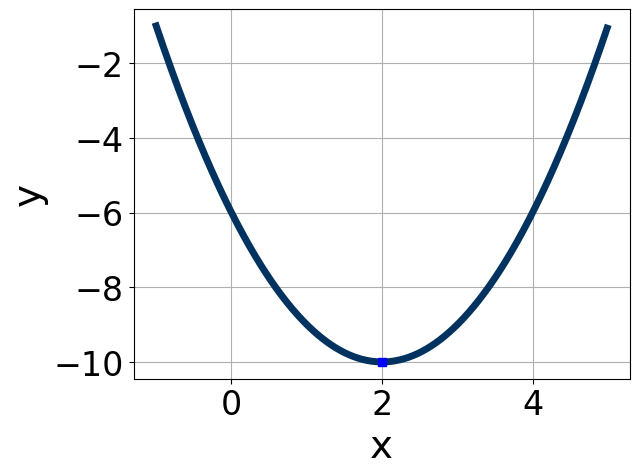
\includegraphics[width=0.5\textwidth]{../Figures/quadraticGraphToEquationB.png}
\end{center}
\begin{enumerate}[label=\Alph*.]
\item \( a \in [-4, 0], \hspace*{5mm} b \in [0, 7], \text{ and } \hspace*{5mm} c \in [-15, -12] \)
\item \( a \in [0, 2], \hspace*{5mm} b \in [-4, -2], \text{ and } \hspace*{5mm} c \in [-8, -4] \)
\item \( a \in [0, 2], \hspace*{5mm} b \in [0, 7], \text{ and } \hspace*{5mm} c \in [14, 17] \)
\item \( a \in [-4, 0], \hspace*{5mm} b \in [-4, -2], \text{ and } \hspace*{5mm} c \in [-15, -12] \)
\item \( a \in [0, 2], \hspace*{5mm} b \in [0, 7], \text{ and } \hspace*{5mm} c \in [-8, -4] \)

\end{enumerate} }
\litem{
Factor the quadratic below. Then, choose the intervals that contain the constants in the form $(ax+b)(cx+d); b \leq d.$\[ 24x^{2} +38 x + 15 \]\begin{enumerate}[label=\Alph*.]
\item \( a \in [-1.31, 1.93], \hspace*{5mm} b \in [13, 22], \hspace*{5mm} c \in [-0.16, 1.34], \text{ and } \hspace*{5mm} d \in [19, 24] \)
\item \( a \in [3.29, 4.95], \hspace*{5mm} b \in [-3, 6], \hspace*{5mm} c \in [5.47, 7.45], \text{ and } \hspace*{5mm} d \in [4, 12] \)
\item \( a \in [6.96, 9.03], \hspace*{5mm} b \in [-3, 6], \hspace*{5mm} c \in [2.25, 4.92], \text{ and } \hspace*{5mm} d \in [4, 12] \)
\item \( a \in [1.81, 2.88], \hspace*{5mm} b \in [-3, 6], \hspace*{5mm} c \in [10.17, 12.99], \text{ and } \hspace*{5mm} d \in [4, 12] \)
\item \( \text{None of the above.} \)

\end{enumerate} }
\litem{
Solve the quadratic equation below. Then, choose the intervals that the solutions $x_1$ and $x_2$ belong to, with $x_1 \leq x_2$.\[ 15x^{2} +38 x + 24 = 0 \]\begin{enumerate}[label=\Alph*.]
\item \( x_1 \in [-1.77, -0.84] \text{ and } x_2 \in [-1.32, -1.11] \)
\item \( x_1 \in [-2.5, -2] \text{ and } x_2 \in [-0.68, -0.61] \)
\item \( x_1 \in [-6.32, -5.86] \text{ and } x_2 \in [-0.46, -0.16] \)
\item \( x_1 \in [-20.14, -19.4] \text{ and } x_2 \in [-18.02, -17.99] \)
\item \( x_1 \in [-2.75, -2.44] \text{ and } x_2 \in [-0.62, -0.44] \)

\end{enumerate} }
\litem{
Write the equation of the graph presented below in the form $f(x)=ax^2+bx+c$, assuming  $a=1$ or $a=-1$. Then, choose the intervals that $a, b,$ and $c$ belong to.
\begin{center}
    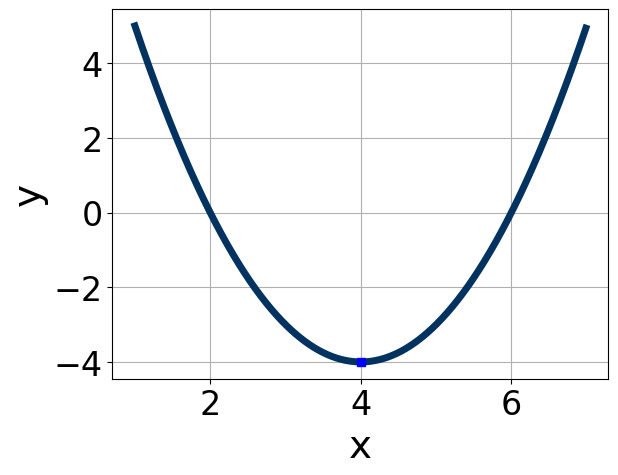
\includegraphics[width=0.5\textwidth]{../Figures/quadraticGraphToEquationCopyB.png}
\end{center}
\begin{enumerate}[label=\Alph*.]
\item \( a \in [0, 2], \hspace*{5mm} b \in [8, 9], \text{ and } \hspace*{5mm} c \in [12, 15] \)
\item \( a \in [0, 2], \hspace*{5mm} b \in [-12, -5], \text{ and } \hspace*{5mm} c \in [12, 15] \)
\item \( a \in [-2, 0], \hspace*{5mm} b \in [-12, -5], \text{ and } \hspace*{5mm} c \in [-22, -18] \)
\item \( a \in [0, 2], \hspace*{5mm} b \in [8, 9], \text{ and } \hspace*{5mm} c \in [20, 22] \)
\item \( a \in [-2, 0], \hspace*{5mm} b \in [8, 9], \text{ and } \hspace*{5mm} c \in [-22, -18] \)

\end{enumerate} }
\litem{
Solve the quadratic equation below. Then, choose the intervals that the solutions belong to, with $x_1 \leq x_2$ (if they exist).\[ 20x^{2} -7 x -2 = 0 \]\begin{enumerate}[label=\Alph*.]
\item \( x_1 \in [-0.96, -0.33] \text{ and } x_2 \in [0, 0.5] \)
\item \( x_1 \in [-0.37, -0.04] \text{ and } x_2 \in [0.2, 1.1] \)
\item \( x_1 \in [-3.87, -3.4] \text{ and } x_2 \in [8.8, 11.1] \)
\item \( x_1 \in [-14.29, -14.01] \text{ and } x_2 \in [12.9, 15.8] \)
\item \( \text{There are no Real solutions.} \)

\end{enumerate} }
\litem{
Factor the quadratic below. Then, choose the intervals that contain the constants in the form $(ax+b)(cx+d); b \leq d.$\[ 36x^{2} -60 x + 25 \]\begin{enumerate}[label=\Alph*.]
\item \( a \in [11.1, 12.9], \hspace*{5mm} b \in [-7, -4], \hspace*{5mm} c \in [1.5, 3.3], \text{ and } \hspace*{5mm} d \in [-7, -3] \)
\item \( a \in [-1.7, 2.2], \hspace*{5mm} b \in [-32, -26], \hspace*{5mm} c \in [-1.2, 2.6], \text{ and } \hspace*{5mm} d \in [-31, -27] \)
\item \( a \in [5.9, 7.2], \hspace*{5mm} b \in [-7, -4], \hspace*{5mm} c \in [5.4, 9.9], \text{ and } \hspace*{5mm} d \in [-7, -3] \)
\item \( a \in [2.4, 4.1], \hspace*{5mm} b \in [-7, -4], \hspace*{5mm} c \in [11.9, 15.7], \text{ and } \hspace*{5mm} d \in [-7, -3] \)
\item \( \text{None of the above.} \)

\end{enumerate} }
\litem{
Graph the equation below.\[ f(x) = -(x+1)^2 - 12 \]\begin{enumerate}[label=\Alph*.]
\begin{multicols}{2}\item 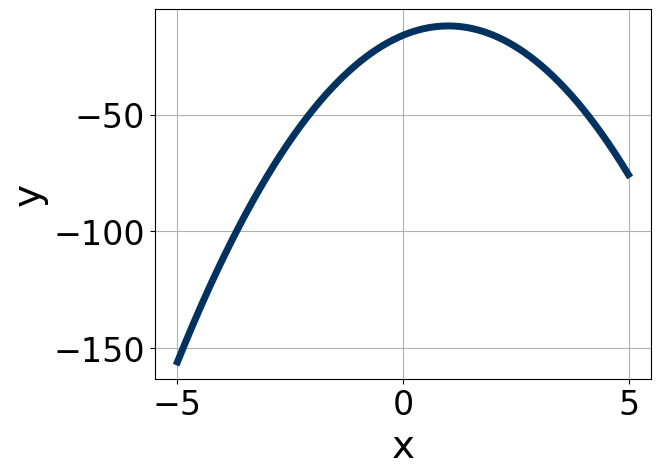
\includegraphics[width = 0.3\textwidth]{../Figures/quadraticEquationToGraphAB.png}\item 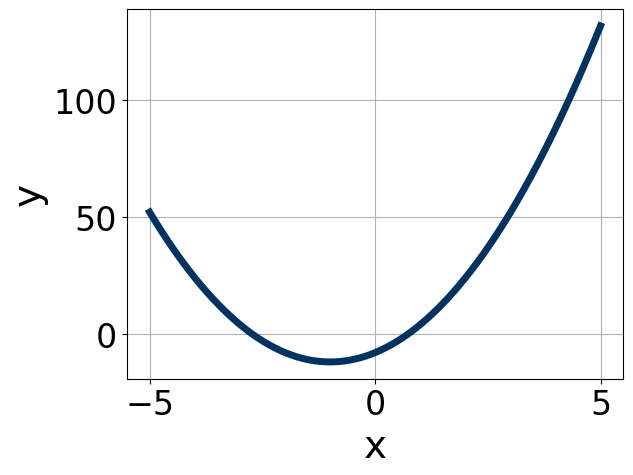
\includegraphics[width = 0.3\textwidth]{../Figures/quadraticEquationToGraphBB.png}\item 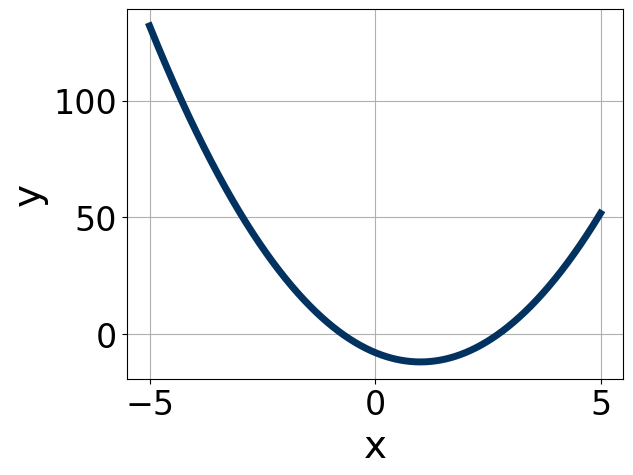
\includegraphics[width = 0.3\textwidth]{../Figures/quadraticEquationToGraphCB.png}\item 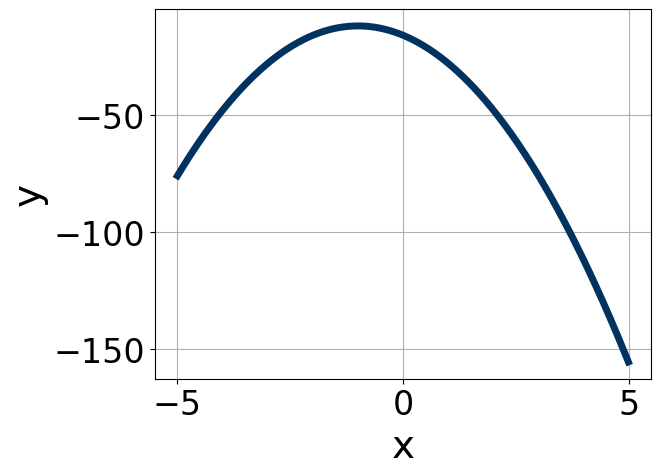
\includegraphics[width = 0.3\textwidth]{../Figures/quadraticEquationToGraphDB.png}\end{multicols}\item None of the above.
\end{enumerate} }
\litem{
Solve the quadratic equation below. Then, choose the intervals that the solutions belong to, with $x_1 \leq x_2$ (if they exist).\[ 14x^{2} -11 x -7 = 0 \]\begin{enumerate}[label=\Alph*.]
\item \( x_1 \in [-2.5, -0.9] \text{ and } x_2 \in [-1.1, 0.9] \)
\item \( x_1 \in [-5.9, -4.1] \text{ and } x_2 \in [15.9, 17.2] \)
\item \( x_1 \in [-22.7, -21.6] \text{ and } x_2 \in [22.9, 25.3] \)
\item \( x_1 \in [-1.2, 1.4] \text{ and } x_2 \in [1, 2.7] \)
\item \( \text{There are no Real solutions.} \)

\end{enumerate} }
\litem{
Solve the quadratic equation below. Then, choose the intervals that the solutions $x_1$ and $x_2$ belong to, with $x_1 \leq x_2$.\[ 15x^{2} -2 x -24 = 0 \]\begin{enumerate}[label=\Alph*.]
\item \( x_1 \in [-6.19, -5.18] \text{ and } x_2 \in [0.25, 0.47] \)
\item \( x_1 \in [-0.78, -0.32] \text{ and } x_2 \in [2.24, 2.79] \)
\item \( x_1 \in [-1.35, -0.62] \text{ and } x_2 \in [0.91, 1.51] \)
\item \( x_1 \in [-2.54, -2.24] \text{ and } x_2 \in [0.48, 0.82] \)
\item \( x_1 \in [-18.5, -17.74] \text{ and } x_2 \in [19.91, 20.15] \)

\end{enumerate} }
\litem{
Graph the equation below.\[ f(x) = -(x+1)^2 - 14 \]\begin{enumerate}[label=\Alph*.]
\begin{multicols}{2}\item 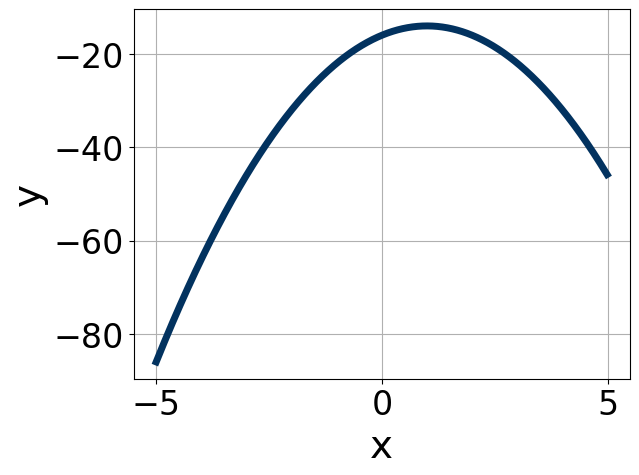
\includegraphics[width = 0.3\textwidth]{../Figures/quadraticEquationToGraphCopyAB.png}\item 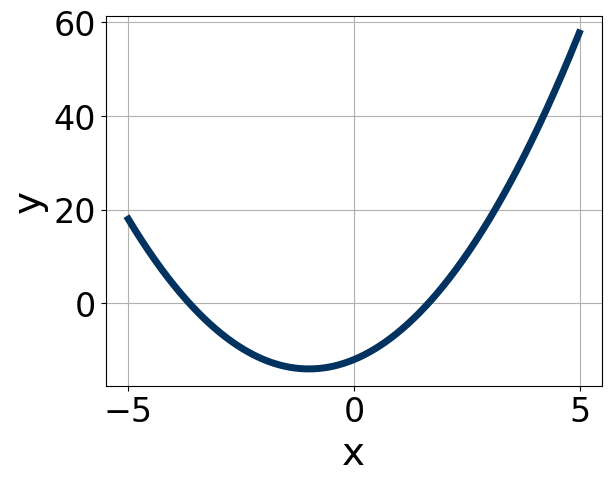
\includegraphics[width = 0.3\textwidth]{../Figures/quadraticEquationToGraphCopyBB.png}\item 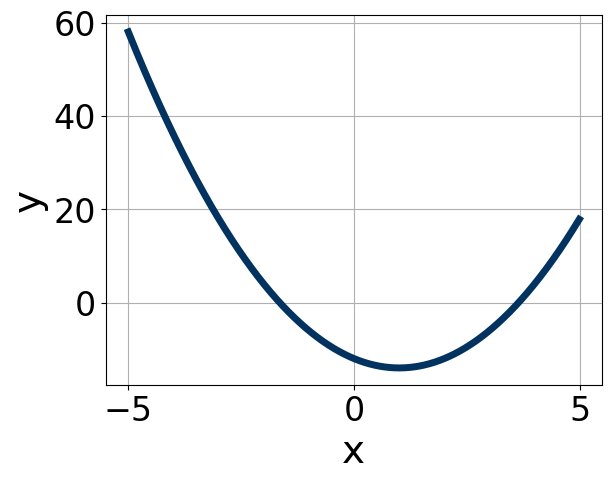
\includegraphics[width = 0.3\textwidth]{../Figures/quadraticEquationToGraphCopyCB.png}\item 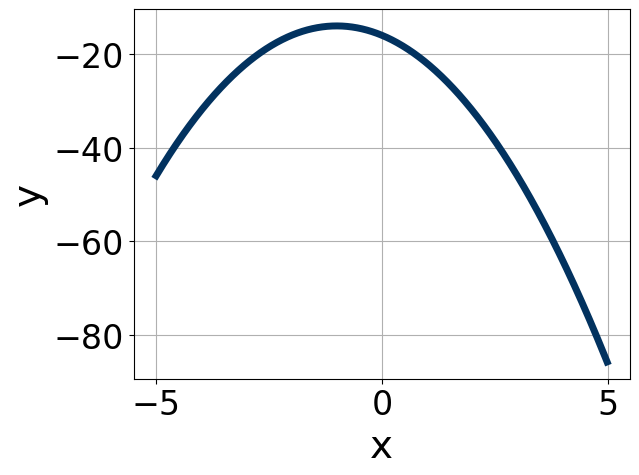
\includegraphics[width = 0.3\textwidth]{../Figures/quadraticEquationToGraphCopyDB.png}\end{multicols}\item None of the above.
\end{enumerate} }
\end{enumerate}

\end{document}